\documentclass[tikz,border=2pt]{standalone}
\usepackage{amsmath,amssymb}
\usepackage{tikz}
\usetikzlibrary{arrows.meta,matrix}

\begin{document}
% An m x n matrix: m rows, n columns, entry a_ij in row i and column j.
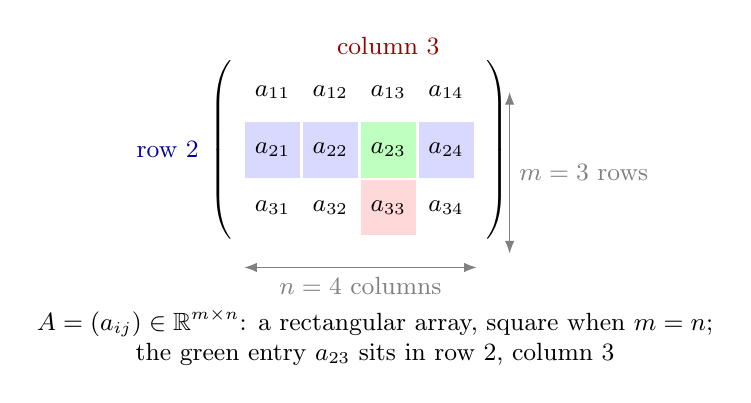
\begin{tikzpicture}[every node/.style={font=\small}, >={Latex[length=1.6mm]}]
	\matrix (A) [matrix of math nodes, nodes={minimum size=7mm, anchor=center}, left delimiter=(, right delimiter=), column sep=1pt, row sep=1pt] at (0,0) {
		a_{11} & a_{12} & a_{13} & a_{14} \\
		|[fill=blue!15]| a_{21} & |[fill=blue!15]| a_{22} & |[fill=green!25]| a_{23} & |[fill=blue!15]| a_{24} \\
		a_{31} & a_{32} & |[fill=red!15]| a_{33} & a_{34} \\
	};
	\node[blue!60!black, font=\small, anchor=east] at ([xshift=-13pt]A-2-1.west) {row $2$};
	\node[red!60!black, font=\small, anchor=south] at (A-1-3.north) {column $3$};
	\draw[<->, gray] (A-1-4.east) ++(0.45,0) -- ++(0,-2.05) node[midway, right, font=\small] {$m=3$ rows};
	\draw[<->, gray] (A-3-1.south west) ++(0,-0.4) -- ++(2.95,0) node[midway, below, font=\small] {$n=4$ columns};
	\node[anchor=north, align=center] at (0.2,-1.9) {$A=(a_{ij})\in\mathbb{R}^{m\times n}$: a rectangular array, square when $m=n$;\\ the green entry $a_{23}$ sits in row $2$, column $3$};
\end{tikzpicture}
\end{document}
